\documentclass{standalone}
\usepackage{tikz}
\begin{document}

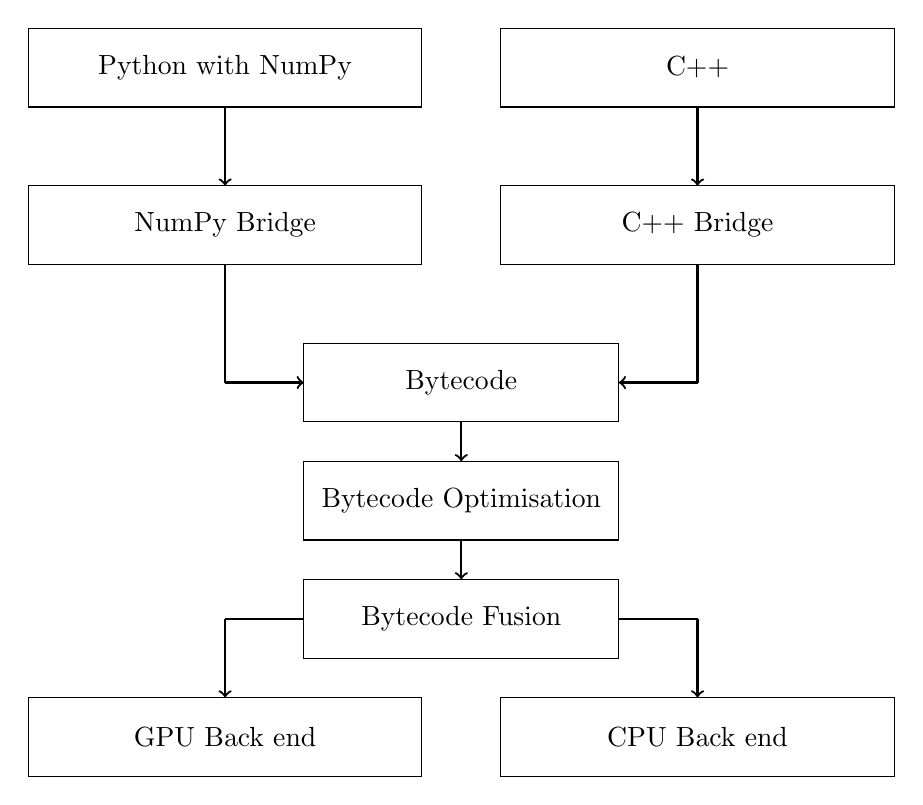
\begin{tikzpicture}
  \draw (1.5,0) rectangle (6.5, 1) node[pos=.5] {Python with NumPy};
  \draw (7.5,0) rectangle (12.5, 1) node[pos=.5] {C++};
  \draw (1.5,-1) rectangle (6.5, -2) node[pos=.5] {NumPy Bridge};
  \draw (7.5,-1) rectangle (12.5, -2) node[pos=.5] {C++ Bridge};

  \draw (5,-3) rectangle (9, -4) node[pos=.5] {Bytecode};
  \draw (5,-4.5) rectangle (9, -5.5) node[pos=.5] {Bytecode Optimisation};
  \draw (5,-6) rectangle (9, -7) node[pos=.5] {Bytecode Fusion};

  \draw (1.5,-7.5) rectangle (6.5, -8.5) node[pos=.5] {GPU Back end};
  \draw (7.5,-7.5) rectangle (12.5, -8.5) node[pos=.5] {CPU Back end};

  \draw[thick, ->] (4, 0) -- (4, -1);
  \draw[thick, ->] (10, 0) -- (10, -1);
  \draw[thick] (4, -2) -- (4, -3.5);
  \draw[thick, ->] (4, -3.5) -- (5, -3.5);
  \draw[thick] (10, -2) -- (10, -3.5);
  \draw[thick, ->] (10, -3.5) -- (9, -3.5);
  \draw[thick, ->] (7, -4) -- (7, -4.5);
  \draw[thick, ->] (7, -5.5) -- (7, -6);

  \draw[thick] (5, -6.5) -- (4, -6.5);
  \draw[thick, ->] (4, -6.5) -- (4, -7.5);

  \draw[thick] (9, -6.5) -- (10, -6.5);
  \draw[thick, ->] (10, -6.5) -- (10, -7.5);

\end{tikzpicture}

\end{document}
